\newif\ifarxiv
\arxivtrue % comment out for BMVC

\ifarxiv
    \documentclass{article}
    \usepackage[margin=1.2in]{geometry}
    \makeatletter
    \newcommand\footnoteref[1]{\protected@xdef\@thefnmark{\ref{#1}}\@footnotemark}
    \makeatother
\else
  \documentclass{bmvc/bmvc2k}
  %% Enter your paper number here for the review copy
  % \bmvcreviewcopy{965}
\fi

% \documentclass{article}

% spacing for editting -------
%\usepackage{setspace}
%\doublespacing
%\onehalfspacing
% spacing for editting -------

% my packages {
%\usepackage{times}
% not sure if these are allowed in CVPR:
\usepackage{bm}
\usepackage{enumitem}
% Definitions of handy macros can go here
%\usepackage{epsfig}
%\usepackage{amsmath}
%\usepackage{amssymb}
%\newcommand{\dataset}{{\cal D}}
%\newcommand{\fracpartial}[2]{\frac{\partial #1}{\partial  #2}}
% Include other packages here, before hyperref.
%\usepackage[breaklinks=true,bookmarks=false]{hyperref}
\usepackage{siunitx}
\usepackage{tikz}
\usetikzlibrary{calc,arrows.meta,positioning,decorations.markings}
\usepackage{amsfonts}
\usepackage{amsmath}

\usepackage[linesnumbered,ruled]{algorithm2e}
%\usepackage[linesnumbered,ruled,vlined]{algorithm2e}
\newcommand\mycommfont[1]{\footnotesize\ttfamily\textcolor{gray}{#1}}
\SetCommentSty{mycommfont}

%\usepackage{siunitx}
%\usepackage{dcolumn,booktabs}
%\newcolumntype{d}[1]{D{.}{.}{#1}}
%\newcommand\mc[1]{\multicolumn{1}{c}{#1}} % handy shortcut macro
%\usepackage[none]{hyphenat} % Inserted this to not have line splits  -'s
%\usepackage{enumitem}
%\usepackage{subcaption}
%\usepackage{gensymb}
%\usepackage{stmaryrd}
%\usepackage{fancyhdr}
%\usepackage{relsize}
% } my packages

% Recommended, but optional, packages for figures and better typesetting:
\usepackage{microtype}
\usepackage{graphicx,calc}
\usepackage{subfigure}
\usepackage{booktabs} % for professional tables

% hyperref makes hyperlinks in the resulting PDF.
% If your build breaks (sometimes temporarily if a hyperlink spans a page)
% please comment out the following usepackage line and replace
% \usepackage{icml2018} with \usepackage[nohyperref]{icml2018} above.
\usepackage{hyperref}

%\usepackage[percent]{overpic}

% Attempt to make hyperref and algorithmic work together better:
\newcommand{\theHalgorithm}{\arabic{algorithm}}

\newlength\myheight
\newlength\mydepth
\settototalheight\myheight{Xygp}
\settodepth\mydepth{Xygp}
\setlength\fboxsep{0pt}
\newcommand*\inlinegraphics[1]{%
  \settototalheight\myheight{Xygp}%
  \settodepth\mydepth{Xygp}%
  \raisebox{-\mydepth}{\includegraphics[height=\myheight]{#1}}%
}

\renewcommand*\ttdefault{lcmtt}
\newcommand\ndash{\mathop{\mbox{$n$-}}}
\newcommand\dashw{\mathop{\mbox{-$\mathsf{w}$}}}
%\newcommand{\TMS}{{\mkern-2mu\times\mkern-2mu}}
\newcommand{\TMS}{{\mkern-1.5mu\times\mkern-1.5mu}}

\newenvironment{tightitemize}
{ \begin{itemize}
    \setlength{\itemsep}{4pt}
    \setlength{\parskip}{0pt}
    \setlength{\parsep}{0pt}     }
{ \end{itemize}                  }

\usepackage{mathtools}
\DeclarePairedDelimiter\ceil{\lceil}{\rceil}
\DeclarePairedDelimiter\floor{\lfloor}{\rfloor}

% Use the following line for the initial blind version submitted for review:
%\usepackage{icml/icml2018}

% If accepted, instead use the following line for the camera-ready submission:
% \usepackage[accepted]{icml/icml2018}

% The \icmltitle you define below is probably too long as a header.
% Therefore, a short form for the running title is supplied here:
% \icmltitlerunning{Knowledge and Techniques Matter}

\begin{document}

%\raggedbottom

\ifarxiv
	\title{A New Benchmark and Progress Toward Improved Weakly Supervised Learning}
	\author{Jason Ramapuram\footnote{Equal contributions.}
          \footnote{University of Geneva \& University of Applied
            Sciences, Western
          Switzerland}\ , jason@ramapuram.net \\ Russ Webb\textsuperscript{*}\footnote{Apple Inc, Cupertino, CA}\ , rwebb@apple.com}
	\maketitle
\else
        % \twocolumn[
        %\icmltitle{Knowledge and Techniques Matter: \\Exploring the Limits of Weakly Supervised Learning}
        %\title{All-Pairs: Benchmarking the Limits of Weakly Supervised Learning}
        %\title{Learned Spatial Histograms and Benchmarking Weakly Supervised Learning}
        %\title{Learned Spatial Histograms to Improve a Benchmarks of Weakly Supervised Learning}
        %\title{Learned Spatial Histograms to Improve Weakly Supervised Learning}
        % A New Benchmark and Improvements for Weakly Supervised Learning
        \title{A New Benchmark and Progress Toward Improved Weakly Supervised Learning}
        % All-Pairs: A Benchmark for Weakly Supervised Learning
        \addauthor{Jason Ramapuram}{jason@ramapuram.net}{2}
        \addauthor{Russ Webb}{rwebb@apple.com}{1}

        % Enter the institutions
        % \addinstitution{Name\\Address}
        \addinstitution{
          Apple Inc\\
          Cupertino, California, USA
        }
        \addinstitution{
          University of Geneva \& \\University of Applied Sciences, \\
          Western Switzerland
        }

        \runninghead{Ramapuram, Webb}{Toward Improved Weakly Supervised Learning}

        % \vskip 0.3in
        % ]
        \maketitle
\fi


% this must go after the closing bracket ] following \twocolumn[ ...

% This command actually creates the footnote in the first column
% listing the affiliations and the copyright notice.
% The command takes one argument, which is text to display at the start of the footnote.
% The \icmlEqualContribution command is standard text for equal contribution.
% Remove it (just {}) if you do not need this facility.

%\printAffiliationsAndNotice{}  % leave blank if no need to mention equal contribution
% \printAffiliationsAndNotice{\icmlEqualContribution} % otherwise use the standard text.

% =========================================================

\begin{abstract}%   <- trailing '%' for backward compatibility of .sty file
{\em Knowledge Matters: Importance of Prior Information for Optimization} \cite{gulccehre2016knowledge}, by G\"{u}l\c{c}ehre et. al.,
sought to establish the limits of current black-box, deep learning
techniques by posing problems which are difficult to learn without engineering
knowledge into the model or training procedure.  In our work, we
solve the previous {\em Knowledge Matters} problem with 100\% accuracy
using a generic model, pose a more
difficult and scalable problem, All-Pairs, and advance this new problem
by introducing a new learned, spatially-varying histogram model called TypeNet which outperforms conventional
models on the problem.  We present results on All-Pairs where our model
achieves 100\% test accuracy while the best ResNet models achieve 79\%
accuracy.  In addition, our model is more than an order of magnitude smaller than Resnet-34.  The challenge of solving larger-scale
All-Pairs problems with high accuracy is presented to the community for investigation.
\end{abstract}

\begin{figure}[t]
\begin{center}
   \includegraphics[width=1.0\linewidth]{figures/nas_comp_v3}
\end{center}
   \vspace{-4mm}
   \caption{The comparison between NetAdaptV2 and related works. The number above a marker is the corresponding total search time measured on NVIDIA V100 GPUs.}
\label{fig:nas_comparison}
\end{figure}

\section{Introduction}
\label{sec:introduction}

Neural architecture search (NAS) applies machine learning to automatically discover deep neural networks (DNNs) with better performance (e.g., better accuracy-latency trade-offs) by sampling the search space, which is the union of all discoverable DNNs. The search time is one key metric for NAS algorithms, which accounts for three steps: 1) training a \emph{super-network}, whose weights are shared by all the DNNs in the search space and trained by minimizing the loss across them, 2) training and evaluating sampled DNNs (referred to as \emph{samples}), and 3) training the discovered DNN. Another important metric for NAS is whether it supports non-differentiable search metrics such as hardware metrics (e.g., latency and energy). Incorporating hardware metrics into NAS is the key to improving the performance of the discovered DNNs~\cite{eccv2018-netadapt, Tan2018MnasNetPN, cai2018proxylessnas, Chen2020MnasFPNLL, chamnet}.


There is usually a trade-off between the time spent for the three steps and the support of non-differentiable search metrics. For example, early reinforcement-learning-based NAS methods~\cite{zoph2017nasreinforcement, zoph2018nasnet, Tan2018MnasNetPN} suffer from the long time for training and evaluating samples. Using a super-network~\cite{yu2018slimmable, Yu_2019_ICCV, autoslim_arxiv, cai2020once, yu2020bignas, Bender2018UnderstandingAS, enas, tunas, Guo2020SPOS} solves this problem, but super-network training is typically time-consuming and becomes the new time bottleneck. The gradient-based methods~\cite{gordon2018morphnet, liu2018darts, wu2018fbnet, fbnetv2, cai2018proxylessnas, stamoulis2019singlepath, stamoulis2019singlepathautoml, Mei2020AtomNAS, Xu2020PC-DARTS} reduce the time for training a super-network and training and evaluating samples at the cost of sacrificing the support of non-differentiable search metrics. In summary, many existing works either have an unbalanced reduction in the time spent per step (i.e., optimizing some steps at the cost of a significant increase in the time for other steps), which still leads to a long \emph{total} search time, or are unable to support non-differentiable search metrics, which limits the performance of the discovered DNNs.

In this paper, we propose an efficient NAS algorithm, NetAdaptV2, to significantly reduce the \emph{total} search time by introducing three innovations to \emph{better balance} the reduction in the time spent per step while supporting non-differentiable search metrics:

\textbf{Channel-level bypass connections (mainly reduce the time for training and evaluating samples, Sec.~\ref{subsec:channel_level_bypass_connections})}: Early NAS works only search for DNNs with different numbers of filters (referred to as \emph{layer widths}). To improve the performance of the discovered DNN, more recent works search for DNNs with different numbers of layers (referred to as \emph{network depths}) in addition to different layer widths at the cost of training and evaluating more samples because network depths and layer widths are usually considered independently. In NetAdaptV2, we propose \emph{channel-level bypass connections} to merge network depth and layer width into a single search dimension, which requires only searching for layer width and hence reduces the number of samples.

\textbf{Ordered dropout (mainly reduces the time for training a super-network, Sec.~\ref{subsec:ordered_droput})}: We adopt the idea of super-network to reduce the time for training and evaluating samples. In previous works, \emph{each} DNN in the search space requires one forward-backward pass to train. As a result, training multiple DNNs in the search space requires multiple forward-backward passes, which results in a long training time. To address the problem, we propose \emph{ordered dropout} to jointly train multiple DNNs in a \emph{single} forward-backward pass, which decreases the required number of forward-backward passes for a given number of DNNs and hence the time for training a super-network.

\textbf{Multi-layer coordinate descent optimizer (mainly reduces the time for training and evaluating samples and supports non-differentiable search metrics, Sec.~\ref{subsec:optimizer}):} NetAdaptV1~\cite{eccv2018-netadapt} and MobileNetV3~\cite{Howard_2019_ICCV}, which utilizes NetAdaptV1, have demonstrated the effectiveness of the single-layer coordinate descent (SCD) optimizer~\cite{book2020sze} in discovering high-performance DNN architectures. The SCD optimizer supports both differentiable and non-differentiable search metrics and has only a few interpretable hyper-parameters that need to be tuned, such as the per-iteration resource reduction. However, there are two shortcomings of the SCD optimizer. First, it only considers one layer per optimization iteration. Failing to consider the joint effect of multiple layers may lead to a worse decision and hence sub-optimal performance. Second, the per-iteration resource reduction (e.g., latency reduction) is limited by the layer with the smallest resource consumption (e.g., latency). It may take a large number of iterations to search for a very deep network because the per-iteration resource reduction is relatively small compared with the network resource consumption. To address these shortcomings,  we propose the \emph{multi-layer coordinate descent (MCD) optimizer} that considers multiple layers per optimization iteration to improve performance while reducing search time and preserving the support of non-differentiable search metrics.

Fig.~\ref{fig:nas_comparison} (and Table~\ref{tab:nas_result}) compares NetAdaptV2 with related works. NetAdaptV2 can reduce the search time by up to $5.8\times$ and $2.4\times$ on ImageNet~\cite{imagenet_cvpr09} and NYU Depth V2~\cite{nyudepth} respectively and discover DNNs with better performance than state-of-the-art NAS works. Moreover, compared to NAS-discovered MobileNetV3~\cite{Howard_2019_ICCV}, the discovered DNN has $1.8\%$ higher accuracy with the same latency.


\section{Related work}
\label{sec:related_work}

Accessibility is an essential component of computing, which aims to make technology broadly accessible to as many users as possible, including those with differing sets of abilities. Improvements in usability and accessibility falls to the community, to better understand the needs of users with differing abilities, and to design technologies that play to this spectrum of abilities \citep{Wobbrock2011AbilityBasedDC}.
In computing, significant strides have been made to increase the accessibility of web content. For example, various versions of the Web Content Accessibility Guidelines (WCAG) \citep{Chisholm2001WebCA, Caldwell2008WebCA} and the in-progress working draft for WCAG 3.0,\footnote{\href{https://www.w3.org/TR/wcag-3.0/}{https://www.w3.org/TR/wcag-3.0/}} or standards such as ARIA from the W3C's Web Accessibility Initiative (WAI)\footnote{\href{https://www.w3.org/WAI/standards-guidelines/aria/}{https://www.w3.org/WAI/standards-guidelines/aria/}} have been released and used to guide web accessibility design and implementation. Similarly, positive steps have been made to improve the accessibility of user interfaces and user experience \citep{Peissner2012MyUIGA, Peissner2013UserCI, Thompson2014ImprovingTU, Bigham2014MakingTW}, as well as various types of media content \citep{Mirri2017TowardsAG, Nengroo2017AccessibleI, Gleason2020TwitterAA}. 

We take inspiration from accessibility design principles in our effort to make research publications more accessible to users who are blind and low vision. Blindness and low vision are some of the most common forms of disability, affecting an estimated 3--10\% of Americans depending on how visual impairment is defined \citep{CDCVisionLossBurden}. BLV researchers also make up a representative sample of researchers in the United States and worldwide. A recent Nature editorial pushes the scientific community to better support researchers with visual impairments \citep{NatureCareerColumn2020}, since existing tools and resources can be limited. There are many inherent accessibility challenges to performing research. In this paper, we engage with one of these challenges that affects all domains of study, accessing and reading the content of academic publications. 

BLV users interact with papers using screen readers, braille displays, text-to-speech, and other assistive tools. A WebAIM survey of screen reader users found that the vast majority (75.1\%) of respondents indicate that PDF documents are very or somewhat likely to pose significant accessibility issues.\footnote{\href{https://webaim.org/projects/screenreadersurvey8/}{https://webaim.org/projects/screenreadersurvey8/}} Most paper are published in PDF, which is inherently inaccessible, due in large part to its conflation of visual layout information with semantic content \citep{NielsenPDFStillUnfit, Bigham2016AnUT}. 
\citet{Bigham2016AnUT} describe the historical reasons we use PDF as the standard document format for scientific publications, as well as the barriers the format itself presents to accessibility. Prior work on scientific accessibility have made recommendations for how to make PDFs more accessible \cite{Rajkumar2020PDFAO, Darvishy2018PDFAT}, including greater awareness for what constitutes an accessible PDF and better tooling for generating accessible PDFs. Some work has focused on addressing components of paper accessibility, such as the correct way for screen readers to interpret and read mathematical equations \citep{Flores2010MathMLTA, Bates2010SpokenMU, Sorge2014TowardsMM, Mackowski2017MultimediaPF, Ahmetovic2018AxessibilityAL, Ferreira2004EnhancingTA, Sojka2013AccessibilityII}, describe charts and figures \citep{Elzer2008AccessibleBC, Engel2017TowardsAC, Engel2019SVGPlottAA}, automatically generate figure captions \citep{Chen2019NeuralCG, Qian2020AFS}, or automatically classify the content of figures \citep{Kim2018MultimodalDL}. Other work applicable to all types of PDF documents aims to improve automatic text and layout detection of scanned documents \cite{Nazemi2014PracticalSM} and extract table content \cite{Fan2015TableRD, Rastan2019TEXUSAU}. In this work, we focus on the issue of representing overall document structure, and navigation within that structure. Being able to quickly navigate the contents of a paper through skimming and scanning is an essential reading technique \citep{Maxwell1972SkimmingAS}, which is currently under-supported by PDF documents and PDF readers when reading these documents by screen reader. 

There also exists a variety of automatic and manual tools that assess and fix accessibility compliance issues in PDFs, including the Adobe Acrobat Pro Accessibility Checker\footnote{\href{https://www.adobe.com/accessibility/products/acrobat/using-acrobat-pro-accessibility-checker.html}{https://www.adobe.com/accessibility/products/acrobat/using-acrobat-pro-accessibility-checker.html}}, Common Look\footnote{\href{https://monsido.com/monsido-commonlook-partnership}{https://monsido.com/monsido-commonlook-partnership}}, ABBYY FineReader\footnote{\href{https://pdf.abbyy.com/}{https://pdf.abbyy.com/}}, PAVE\footnote{\href{https://pave-pdf.org/faq.html}{https://pave-pdf.org/faq.html}}, and PDFA Inspector\footnote{\href{https://github.com/pdfae/PDFAInspector}{https://github.com/pdfae/PDFAInspector}}. To our knowledge, PAVE and PDFA Inspector are the only non-proprietary, open-source tools for this purpose. Based on our experiences, however, all of these tools require some degree of human intervention to properly tag a scientific document, and tagging and fixing must be performed for each new version of a PDF, regardless of how minor the change may be.

Guidelines and policy changes have been introduced in the past decade to ameliorate some of the issues around scientific PDF accessibility. Some conferences, such as The ACM CHI Virtual Conference on Human Factors in Computing Systems (CHI) and The ACM SIGACCESS Conference on Computers and Accessibility (ASSETS), have released guidelines for creating accessible submissions.\footnote{See \href{http://chi2019.acm.org/authors/papers/guide-to-an-accessible-submission/}{http://chi2019.acm.org/authors/papers/guide-to-an-accessible-submission/} and \href{https://assets19.sigaccess.org/creating_accessible_pdfs.html}{https://assets19.sigaccess.org/creating\_accessible\_pdfs.html}} The ACM Digital Library\footnote{\href{https://dl.acm.org/}{https://dl.acm.org/}} provides some publications in HTML format, which is easier to make accessible than PDF~\cite{Graells2007EstudioDL}. \citet{Ribera2019PublishingAP} conducted a case study on DSAI 2016 (Software Development and Technologies for Enhancing Accessibility and Fighting Infoexclusion). The authors of DSAI were responsible for creating accessible proceedings and identified barriers to creating accessible proceedings, including lack of sufficient tooling and lack of awareness of accessibility. The authors recommended creating a new role in the organizing committee dedicated to accessible publishing. These policy changes have led to improvements in localized communities, but have not been widely adopted by all academic publishers and conference organizers.

Table~\ref{tab:prior_work} lists prior studies that have analyzed PDF accessibility of academic papers, and shows how our study compares. Prior work has primarily focused on papers published in Human-Computer Interaction and related fields, specific to certain publication venues, while our analysis tries to quantify paper accessibility more broadly.
\citet{Brady2015CreatingAP} quantified the accessibility of 1,811 papers from CHI 2010-2016, ASSETS 2014, and W4A, assessing the presence of document tags, headers, and language. They found that compliance improved over time as a response to conference organizers offering to make papers accessible as a service to any author upon request. \citet{Lazar2017MakingTF} conducted a study quantifying accessibility compliance at CHI from 2010 to 2016 as well as ASSETS 2015,
%\jb{Define acronyms in prev para}
confirming the results of \citet{Brady2015CreatingAP}. They found that across 5 accessibility criteria, the rate of compliance was less than 30\% for CHI papers in each of the 7 years that were studied. The study also analyzed papers from ASSETS 2015, an ACM conference explicitly focused on accessibility, and found that those papers had significantly higher rates of compliance, with over 90\% of the papers being tagged for correct reading order and no criteria having less than 50\% compliance. This finding indicates that community buy-in is an important contributor to paper accessibility.
\citet{Nganji2015ThePD} conducted a study of 200 PDFs of papers published in four disability studies journals, finding that accessibility compliance was between 15-30\% for the four journals analyzed, with some publishers having higher adherence than others. To date, no large scale analysis of scientific PDF accessibility has been conducted outside of disability studies and HCI, due in part to the challenge of scaling such an analysis. We believe such an analysis is useful for establishing a baseline and characterizing routes for future improvement. Consequently, as part of this work, we conduct an analysis of scientific PDF accessibility across various fields of study, and report our findings relative to prior work. 


\begin{table}[t!]
\small
    \centering
    \begin{tabularx}{\linewidth}{L{22mm}L{15mm}L{48mm}L{16mm}L{34mm}}
        \toprule
        \textbf{Prior work} & \textbf{PDFs analyzed} & \textbf{Venues} & \textbf{Year} & \textbf{Accessibility checker} \\
        \midrule
        \citet{Brady2015CreatingAP} & 1811 & CHI, ASSETS and W4A & 2011--2014 & PDFA Inspector \\ [0.5mm]
        \hline \\ [-2.5mm]
        \citet{Lazar2017MakingTF} & 465 + 32 & CHI and ASSETS & 2014--2015 & Adobe Acrobat Action Wizard \\ [0.5mm]
        \hline \\ [-2.5mm]
        \citet{Ribera2019PublishingAP} & 59 & DSAI & 2016 & Adobe PDF Accessibility Checker 2.0 \\ [0.5mm]
        \hline \\ [-2.5mm]
        \citet{Nganji2015ThePD} & 200 & \textit{Disability \& Society}, \textit{Journal of Developmental and Physical Disabilities}, \textit{Journal of Learning Disabilities}, and \textit{Research in Developmental Disabilities} & 2009--2013 & Adobe PDF Accessibility Checker 1.3 \\ [0.6mm]
        \hline \\ [-2.5mm]
        \textbf{\textit{Our analysis}} & \numpdfs & Venues across various fields of study & 2010--2019 & Adobe Acrobat Accessibility Plug-in Version 21.001.20145 \\
        \bottomrule
    \end{tabularx}
    \caption{Prior work has investigated PDF accessibility for papers published in specific venues such as CHI, ASSETS, W4A, DSAI, or various disability journals. Several of these works were conducted manually, and were limited to a small number of papers, while the more thorough analysis was conducted for CHI and ASSETS, two conference venues focused on accessibility and HCI. Our study expands on this prior work to investigate accessibility over \numpdfs PDFs sampled from across different fields of study.
    }
    % \Description{
    % Prior work, PDFs analyzed, Venues, Year, Accessibility checker 
    % Brady et al. [7], 1811, CHI, ASSETS and W4A, 2011--2014, PDFA Inspector 
    % Lazar et al. [23], 465 + 32, CHI and ASSETS, 2014--2015, Adobe Acrobat Action Wizard 
    % Ribera et al. [40], 59, DSAI, 2016, Adobe PDF Accessibility Checker 2.0 
    % Nganji [33], 200, Disability & Society, Journal of Developmental and Physical Disabilities, Journal of Learning Disabilities, and Research in Developmental Disabilities, 2009--2013, Adobe PDF Accessibility Checker 1.3
    % Our analysis, 11397, Venues across various fields of study, 2010--2019, Adobe Acrobat Accessibility Plug-in Version 21.001.20145 
    % }
    \label{tab:prior_work}
\end{table}
% ==================================================
\section{Solving the Pentomino Problem}
% -----------------------------------
% -----------------------------------

\begin{figure*}[!htb]
\minipage[t]{0.468\textwidth}
  \includegraphics[width=\linewidth]{images/pentomino}
  \endminipage\hfill
\minipage[t]{0.532\textwidth}
  \includegraphics[width=\linewidth]{images/km_solved.png}
\endminipage\hfill
\caption{\emph{Left}: The Pentomino sprites and two examples illustrating the $true$ and $false$ classes.
  \emph{Right}: Test accuracy (median and inner quartiles, 10 trials) on the Pentomino problem with and without modern training advances. Note, log-scale of x-axis.}
\label{pento_sprites}
\end{figure*}

{\em Knowledge Matters} \cite{gulccehre2016knowledge} explores the extent to
which neural networks are able to learn problems given minimal
supervised information. Their formulation has a fully defined loss
function; however, the gradient of the loss with respect to the
parameters provides no direct information about potentially useful
subtasks such as segmentation, object classification, or counting. They concluded that the networks and training methods they tested converged to a
local minima.

The {\em Knowledge Matters} demonstration utilized the Pentomino dataset, which
is formed from a set of sprites \cite{gulcehre_2015}
shown in Figure \ref{pento_sprites}. The
dataset is generated by placing three sprites onto a canvas $C \in
\mathbb{R}^{64\TMS64}$. Each sprite undergoes a random rotation 
(\ang{0}, \ang{90}, \ang{180}, or \ang{270}) and integer scaling ($1\times$ or $2\times$).  The goal of the
neural network is to predict a 1 if the rotated and scaled sprites in an
image are the same and 0 otherwise. One possible solution to the
Pentomino problem is to learn to segment, classify, and count the number
of underlying objects in the image. The challenge (claimed impossible in \cite{gulcehre_2015})
is to find a solution using a generic network given only the binary
label for each image.

G\"{u}l\c{c}ehre et. al \cite{gulccehre2016knowledge} observed that
``black-box machine  learning  algorithms  could  not  perform  better 
than  chance on [the Pentomino problem].'' Decomposing
the problem into two stages however, made the task easily solvable. The
first stage in the decomposition was a classification
step, where extra label information was provided to the model. Given the
predicted classes, the second stage projected this output to the Bernouili
log-likelihood objective. Using some of the recent advances in 
DNN training, we are able to completely solve the original
problem demonstrated in {\em Knowledge Matters}; we do so without the
requirement of an intermediary model or the addition of extra
information. We also experimented with a reproduction of the model 
proposed in the paper and found that given enough time (over 1000
epochs) the model does make progress on the Pentomino problem, as shown
in Figure \ref{pento_sprites} in gray. This observation is in line with
recent insights of \cite{hoffer2017train} that discuss the effects of
training duration and batch size.

The fully-connected (fc) model presented in \cite{gulccehre2016knowledge} was composed of layer sizes
[2050, 11, 1024] and trained with ADADelta \cite{zeiler2012adadelta} and weight regularization. The 11-unit layer
served as a bottleneck to bring structural information into the
network.  We leverage four recent advances to solve the Pentomino problem: Batch
Normalization (BN) \cite{ioffe2015batch}, Exponential Linear Units
\cite{clevert2015fast}, the Adam optimizer \cite{kingma2014adam}, and
Xavier initializations \cite{glorot2010understanding}. In constrast to
the large model employed in \cite{gulccehre2016knowledge}, we use a
fully-connected network with layer sizing of
$[32, 64, 12, 32, 8]$; this translates to a 98.5\% reduction of the
total number of model parameters. Comparable in size to the largest
training sets used in \cite{gulccehre2016knowledge}, 486k
samples were used for training and 54k samples were held out for testing.

G\"{u}l\c{c}ehre et. al \cite{gulccehre2016knowledge} were only able to
train black-box (generic), fully-connected models to achieve 50\% accuracy on the
Pentomino dataset. Their best model, after significant
hyper-parameter search, resulted in a 5.3\% training and 6.7\% test error
on the 80k Pentomino training dataset. This performance was achieved 
via a two-stage network that induced structural information
into the neural network. On the same training set, we achieved a 1\% error using a black-box neural network with the
5-layer network described above.  Figure
\ref{pento_sprites} shows the training accuracy for the original
{\em Knowledge Matters} network (gray), our modification (blue), and our TypeNet model (green, see Section \ref{typenetdetails}) on
the Pentomino problem (note the log scale on the x-axis).

%%% Local Variables:
%%% mode: latex
%%% TeX-master: "0.knowledge_and_techniques_matter"
%%% End:

% ==================================================
\section{The All-Pairs Problem} \label{all_pairs}
% -----------------------------------
\begin{figure}[h!]
\vskip 0.2in
\begin{center}
\scalebox{0.6}{\centerline{\includegraphics[width=\columnwidth]{images/all_pairs_survey}}}
\caption{All-Pairs examples from 2-2 on the left to 8-8 on the right.  The bottom row is $true$ and the top row is $false$.}
\label{example8}
\end{center}
\vskip -0.2in
\end{figure}


\subsection{Definition and Examples}

Extending the ideas in the Pentomino problem, we use anti-aliased white
symbols on a black background to construct the following new problem.
The \textit{N-K} All-Pairs problem contains \textit{2N} symbols from an
alphabet of \textit{K} choices.  Each example is \textit{true} if each of its
symbols pairs with a symbol of the same type without reuse,
and \textit{false} otherwise.  Symbols are positioned randomly with no
overlap.  Symbols are of similar scales, ranging from
10--18 pixels across, and have differing symmetries (for instance, some
are rotationally invariant, while others are not).  The exact structure
and variations of each symbol are given by the generator code supplied
online \cite{allpairs2018}.

Each symbol is shown below with the
number of unique ways it can appear, as configured in our experiments.  In contrast, the
Pentomino problem used 8
variations for each symbol. The symbols are used in the order given, so the 4-4 All-Pairs problem will use \textbf{circle}, \textbf{line}, \textbf{cross}, and \textbf{angle}.  For this work a $76\TMS76$ image is used for $N<6$ and a
$96\TMS96$ image is used for larger $N$.

\begin{table}[htp]
  \begin{center}
\scalebox{0.9}{
\begin{tabular}{r r l r r r l r}
id & name & examples & cardinality &id & name & examples & cardinality \\
\hline
1 & \textbf{circle}        & \inlinegraphics{images/strip_0.png}  & 165   & 10 & \textbf{box}          & \inlinegraphics{images/strip_9.png}  & 480   \\
2 & \textbf{line}          & \inlinegraphics{images/strip_1.png}  & 174   & 11 & \textbf{box-diagonal} & \inlinegraphics{images/strip_10.png} & 518   \\
3 & \textbf{cross}         & \inlinegraphics{images/strip_2.png}  & 45.3k & 12 & \textbf{barbell}      & \inlinegraphics{images/strip_11.png} & 78    \\
4 & \textbf{angle}         & \inlinegraphics{images/strip_3.png}  & 39k   & 13 & \textbf{dot-line}     & \inlinegraphics{images/strip_12.png} & 156   \\
5 & \textbf{3-star}        & \inlinegraphics{images/strip_4.png}  & 1.43M & 14 & \textbf{z}            & \inlinegraphics{images/strip_13.png} & 518   \\
6 & \textbf{theta}         & \inlinegraphics{images/strip_5.png}  & 20k   & 15 & \textbf{triangle-lid} & \inlinegraphics{images/strip_14.png} & 1036  \\
7 & \textbf{phi}           & \inlinegraphics{images/strip_6.png}  & 20k   & 16 & \textbf{dot-mid-line} & \inlinegraphics{images/strip_15.png} & 78    \\
8 & \textbf{2-circle}      & \inlinegraphics{images/strip_7.png}  & 7k& 17 & \textbf{hourglass}    & \inlinegraphics{images/strip_16.png} & 518   \\
9 & \textbf{circle-3star}  & \inlinegraphics{images/strip_8.png}  & 7.15M& 18 & \textbf{triangle}     & \inlinegraphics{images/strip_17.png} & 11.8k \\
\end{tabular}
}
\end{center}
\label{default}
\end{table}
\vskip -0.2in

\noindent
Figure \ref{example8} shows a \textit{true} and a \textit{false} example
for the 2-2 to 8-8 All-Pairs problem.  A data generator for All-Pairs is
used to generate on-demand, unique training examples (the 4-4
All-Pairs problem has approximately $10^{28}$ unique images), and a fixed
validation set is generated at the start of training.  The separability of the eighteen
symbols was confirmed by training a simple conv-net to 100\% test accuracy in 350k training samples.

\subsection{Comparison with Conventional Results}
Conventional algorithms from the literature have difficulty with the 4-4
All-Pairs problem, as shown in the following table.  Clearly, of the
hundreds of conventional, valuable DNN algorithms, there may exist some
that can solve the 4-4 problem.  One open challenge is to identify them
and extend training techniques to efficiently solve these types of problems.
Of the runs of each algorithm summarized below, none achieved more than
92\% test accuracy after training on 100M samples.  An expert human made one mistake in 100 samples for each of the All-Pairs problem from difficulty 4-4 to 7-7, taking 8-9 seconds to classify each image.  Humans use sequential attention and working memory to do the All-Pairs task, suggesting the task as a benchmark for building sequential models.
TypeNet consistently achieves 100\% test accuracy in the 4-4 All-Pairs
problem using 20k test samples.  

\begin{center}
\begin{tabular}{ c c c c c }
 algorithm & model size & normalized size & accuracy & std deviation \\
\hline
 TypeNet [$\times$10] & 918k & 1.0 & \textbf{1.000} & \textbf{0.000} \\
 Expert Human [$\times$1] & -- & -- & \textbf{0.990} & -- \\
 Relational Net [$\times$10] & \textbf{630k} & \textbf{0.7} & 0.867 & 0.078 \\
 \ifarxiv
 ConvNet (\S\ref{comptocnn}) [$\times$4] & 9.9M & 11 & 0.808 & 0.093    \\
 \fi
 Inception v3 [$\times$10] & 22M & 24 & 0.803 & 0.079    \\
 Resnet-34 [$\times$10] & 21M & 23 & 0.788 & 0.068   \\
 Resnet-18 [$\times$10] & 11M & 12 & 0.711 & 0.157    \\
 Vgg19 [$\times$6] & 139M & 151 & 0.509 & 0.002    \\
 Vgg16 [$\times$3] & 134M & 146 & 0.506 & 0.002    \\
\end{tabular}
\end{center}

% ==================================================
\section{Toward an All-Pairs Solution}
% -----------------------------------

\begin{algorithm}
\label{tn_algo_block}
\caption{TypeNet algorithm}
\SetAlgoNoEnd
\SetKwComment{tcp}{\# }{}
    %\KwIn{An image, \textsc{Image}}
    %\KwOut{Model prediction}
    \KwData{ 
    	\begin{itemize}
		\renewcommand\labelitemi{--}
		\setlength\itemsep{-0.2em}
		\item Number of layers, $N_c$ and $N_f$.
		\item Number of type branches, $N_t$, and spatial branches, $N_s$.
		\item Activations, \textsc{Ac}, and convolutions, \textsc{Conv}, for feature extraction layers.
		\item Activations, \textsc{A}, and $n$ 1x1 convolutions, \textsc{Conv1$\TMS$1}, for type matching.
		\item Spatial diversity operations, \textsc{Spatial}.
		\item Activations, \textsc{Afc}, weights, $W$, and biases, $B$, for fully-connected layers.
	\end{itemize}
    }
    %\underline{function TypeNet(\textsc{Image})} \\

$C = \textsc{Image}$ \tcp*[f]{convolution block} \\
\For{$i=[1 \to N_c)$}{
	$C = \textsc{Ac}_i(\textsc{Conv}_i(C))$ \\
	$C = \textsc{BatchNorm}(C)$
}
\BlankLine
T = $\sum_{i=0}^{N_t}{\textsc{A}_i(\textsc{Conv1$\TMS$1}_i(C))}$
\BlankLine
Y = \textsc{Concatenate}\Big(\big[ $\sum_{w,h}{\textsc{Spatial}_i(T)}$ for $i = [0 \to N_s)$ \big]\Big)

\BlankLine
\For(\tcp*[f]{fully-connected layers}){$i=[0 \to N_f)$} { 
	$Y = \textsc{Afc}_i(W_i Y + B_i)$ \\
	$Y = \textsc{BatchNorm}(Y)$
}

\KwRet{$\textsc{SoftMax}(Y)$}
\end{algorithm}

%\tikzstyle{vertex}=[auto=left,circle,fill=black!25,minimum size=20pt,inner sep=0pt]

%\begin{tikzpicture}
%  \node(n4)  at (3,4)  {$n_4$};
%  \node (n5)  at (3,6)  {$n_5$};
%
%
%  \path (n4) -- (n5) node [red, font=\Huge, midway, sloped] {$\dots$};
%
%\end{tikzpicture}

\subsection{Type-Net Model} \label{typenetdetails}

After verifying that a fully-connected model can easily solve the 4-4 All-Pairs
problem from the histogram of symbols in each
image, we designed and tested a generic model capable of
learning a similar, whole-image statistic.  The resulting model was created
using insights derived from the All-Pairs problem, but does not make use of
explicit problem details or enhanced training data.

We refer to the resulting network as a TypeNet because it estimates the affinity
of each receptive field to $n$ ideal types (via a dot-product) and then
aggregates those type-affinities over the spatial extent.  This spatial
summation is global for solving the All-Pairs problem, but could
be spatially restricted to produced learned features similar to
histogram of gradients (HOG) found in \cite{mcconnell1986method}.  A learned attention mask could also generalize the summation to salient areas of each image.

Model details can be found in the supplementary material and in the online sample code found at \cite{allpairs2018}.  The general algorithm for TypeNet is presented in Algorithm \ref{tn_algo_block}.  The algorithm begins and ends conventionally with a convolution stack and fully-connected layers, respectively.  Lines 5 and 6 show the key steps for the algorithm:
\begin{itemize}
\item line 5, the $1\TMS$1 convolution implements a dot-product similarity with a learned kernel, these are the ``types'' of TypeNet.
\item line 5, the activation, \textsc{A}$_i$, applied was experimentally studied:
	\begin{itemize}
	\item \textsc{A}$_i$ = \textsc{SoftMax} in the feature dimension, gives a soft $N_t$-hot representation here which was seen to reduce variance in training times).
	\item \textsc{A}$_i$ = \textsc{Identity} was the most versatile activation and can be seen as creating a ``type'' difference operator
	\end{itemize}
\item line 5, superposition (via summation) of learned template matching
\item line 6, diversify spatially with non-linear operators such as \textsc{MaxPool}.
\end{itemize}

The goal of introducing TypeNet is to expand the palette of
techniques available to solve similar types of problems and decrease
the problem specific reasoning required in similar
domains (such as parity, counting, holistic scene understanding, and
visual query answer), which can be solved from a histogram-like summary of
local statistics.

\subsection{Contrast to Relational Methods}

Relational neural learning generally accomplishes it's goal by
learning a functional over $(i,j)$ tuples in a latent feature space $f$. In
Relational Networks \cite{santoro2017simple} for example, the
model learns two functionals $[h, g]$ (parameterized by
deep-neural networks) that \textbf{exhaustively} operate over \textbf{all} $(i,j)$ pairs
in the latent feature space of a deep-convolutional network as shown
in the table below.
Memory Networks \cite{weston2014memory} on the other hand learn a probabilistic relationship
between the input query (embedded into a feature representation) $f_i$ and an
associated set of memory vectors $M = \{m_1, ... m_i, m_N \}$, followed by a smoothed weighting against an embedded query
vector $c_i$.
% $p_i = \text{softmax}(f_i, m_i) ;  o_i = \sum_i p_i c_i$.
% \vskip -0.2in
% \begin{align}
%   p_i = \text{softmax}(f_i, m_i) \hspace{1in}    o_i = \sum_i p_i c_i
    %   \end{align}
\vskip -0.2in
{\renewcommand{\arraystretch}{1.15}
\begin{center}
\begin{tabular}{ c | c } \hline
  Relational Networks & Memory Networks \\ \hline
  $g(\sum_i \sum_j h(f_i, f_j))$ & $p_i = \text{softmax}(f_i^T,
                                         m_i) \hspace{0.2in}    o_i =
                                         \sum_i p_i c_i$
\end{tabular}\label{rel_mem_net}
\end{center}
}                                     


Relational Networks \cite{santoro2017simple} have high computational
complexity when the dimensionality of the feature-space
$f$ is large. Memory-networks on the other hand scale proportionate
to the number of embedded memories dim($M$). Our objective with TypeNet
is twofold: relax computational constraints compared to these relational models and incorporate the probabilistic smoothing of Memory Networks \cite{weston2014memory}.

We reduce the computational complexity by forcing the model to divide
the input representation through a set of $N_t$ branches. This
division allows the model to learn a disparate feature
representation per branch. Rather than learning over every $(i,j)$ as in Relational Networks \cite{santoro2017simple} we
approximate this with a spatial sum after our branch-divide
strategy.

During our branching strategy we do a sum across an activated feature
space; this can be interpreted as a probabilistic weighting of the
features of each individual branch against each other. Training TypeNet to convergence is \textbf{8-10 times faster} than training a comparable Relational Network and produces \textbf{more accurate results} in the
weak-supervised learning scenario of All-Pairs.

\subsection{All-Pairs Result} \label{allpairsresult}

\begin{figure*}[!htb]
  \includegraphics[width=\linewidth]{images/unified}
\caption{Training results, showing validation accuracy and total number of training sample for TypeNet on increasingly difficult versions of All-Pairs, from 4-4 to 7-7.  Shading shows the distribution over 10 trials.  Note, conventional DNN models cannot solve the 4-4 problem.}
\label{solving_all_pairs}
\end{figure*}

As described, the TypeNet for the All-Pairs problem has 1.04M trainable parameters
(many times smaller than the baseline models).
Unless otherwise noted, we used the following training setup for the
TypeNet results on the All-Pairs problem: 4 GPUs, batch size 600, Adam
with learning rate = 0.001 and no weight decay, cross-entropy loss, test
results reported every 50k training samples, and 100M total training samples.
A 100M sample training run typically takes 20 hours on 4$\TMS$P100 GPUs.

The main hyper-parameters and architecture-variations explored are the
feature activation, number of branches ($k$), and number of features
($n$).  Details of those studies can be found in the supplementary material.  We concluded that $k = 2$ and $n = 64$ performed well on the All-Pairs problem.  Increasing the number of features to 96 results in slightly lower training times, at a cost of a larger model.  All options explored reached 100\% accuracy.

The TypeNet approach cannot easily solve every All-Pairs
problem; Figure \ref{solving_all_pairs} shows results for the 4-4 to 7-7 All-Pairs problem.
We see an increase in the magnitude and variance of the number of samples needed for convergence.  The plot shows the results of 10 training runs for each difficulty level; TypeNet can solve the first 3 of these challenges to 100\% validation accuracy.  No model and training methodology has been found that solves the 7-7 problem to 100\% accuracy.  An inspection of the errors made by the best 7-7 solution shows that they are systematic, unambiguous errors.


\begin{figure*}[!htb]
\centering
\minipage{0.6\textwidth}
  \includegraphics[width=\linewidth]{images/train_sizedata}
\endminipage\hfill
\caption{Training the TypeNet on 4-4 All Pairs with 100M samples drawn from a fixed-size training set.}
\label{data_setsize_fig}
\end{figure*}


% ------------------------
\subsection{Training Set Size}

In Figure \ref{data_setsize_fig}, we show the effect of reducing the
cardinality of the training data from effectively infinite to sizes
smaller than the total number of training samples presented.  A training
set cardinality of 100k is minimal for 90\% test accuracy and 500k is
minimal for some trials to reach 100\% test accuracy.  The increased variance in both train and test accuracy at
cardinality 30k is interesting.  We hypothesize this is due to sampling
noise for these small sizes leading to significantly different train and
test distributions.  For larger cardinality, both sets consistently
represent the same distribution; for smaller sets, learning is
limited enough that distribution differences are not apparent.

To avoid the overhead of datasets on disk, varying the training set
cardinality is accomplished using an array of seeds for the data
generator.  Each seed is used to generate 1k samples.  When each seed in
the list has been used once, the list is shuffled and the process
starts back at the beginning of the list.

%\raggedbottom
%\vfill
\subsection{Other Applications}

TypeNet was evaluated on other datasets to determine its applicability
to common classification problems.  The following table presents results for the test
accuracy from four training runs.  For training, each dataset was augmented by random original-size
crops (padding of 4), random rotations from \ang{0} to \ang{4}, and normalized by subtracting 0.5.
CIFAR10 and Fashion MNIST \cite{fashionref}
were also augmented with random horizontal flips.  A detailed discussion and comparison with a simple convolutional net can be found in Supplement \ref{comptocnn}.

\begin{center}
\begin{tabular}{ r | c c | c c  }
              & \multicolumn{2}{c|}{ConvNet}                        & \multicolumn{2}{c}{TypeNet}  \\
dataset  & accuracy & \# parameters & accuracy & \# parameters \\
\hline
MNIST               & 0.9953 $\pm$ 0.0002    & 2M & \textbf{0.9971 $\pm$ 0.0006} & \textbf{1M}  \\
Fashion-MNIST & \textbf{0.9409 $\pm$ 0.0005}    & 2M & 0.9346 $\pm$ 0.0011 & \textbf{1M} \\
CIFAR10           & 0.7773 $\pm$ 0.0013     & 2.5M & \textbf{0.8820 $\pm$ 0.0080} & \textbf{1M} \\
4-4 All-Pairs      & 0.8080 $\pm$ 0.0925     & 9.9M & \textbf{1.0000 $\pm$ 0.0000} & \textbf{1M} \\
\end{tabular}
\end{center}

%\begin{center}
%\begin{tabular}{ l c c l }
%dataset  & accuracy & stdev \\
%\hline
%MNIST  & 0.9971 & 0.0006  \\
%Fashion-MNIST & 0.9346 & 0.0011 \\
%CIFAR10 & 0.882 & 0.008 \\
%\end{tabular}
%\end{center}

For these classification
tasks, adding more spatial information via two parallel pathways branching
from the \textbf{similarity} step (algorithm line 5) and joining at the \textbf{concatenation} step (line 6)
was useful.  One of these extra pathways has a \textsc{MaxPool3x3} and the other has \textsc{AvgPool3x3} after
the \textbf{similarity} step.  This enhanced model also solves the All-Pairs problem and has 10\% more parameters than the simpler TypeNet presented as a minimal version for All-Pairs.

 We propose a novel commonsense reasoning challenge, \textsc{RiddleSense}, which requires complex commonsense skills for reasoning about creative and counterfactual questions, coming with a large multiple-choice QA dataset.  
 We systematically evaluate recent commonsense reasoning methods over the proposed \textsc{RiddleSense} dataset, and find that the best model is still far behind human performance, suggesting that there is still much space for commonsense reasoning methods to improve.
 We hope \textsc{RiddleSense} can serve as a benchmark dataset for future research targeting complex commonsense reasoning and computational creativity.


\section*{Acknowledgements}
This research is supported in part by the Office of the Director of National Intelligence (ODNI), Intelligence Advanced Research Projects Activity (IARPA), via Contract No. 2019-19051600007, the DARPA MCS program under Contract No. N660011924033 with the United States Office Of Naval Research, the Defense Advanced Research Projects Agency with award W911NF-19-20271, and NSF SMA 18-29268. The views and conclusions contained herein are those of the authors and should not be interpreted as necessarily representing the official policies, either expressed or implied, of ODNI, IARPA, or the U.S. Government. We would like to thank all the collaborators in USC INK research lab and the reviewers for their constructive feedback on the work.
%\input{full_diagram}

\ifarxiv
    %\bibliographystyle{alpha}
    \bibliographystyle{abbrv}
\fi

\bibliography{0_Progress_Toward_Improved_Weakly_Supervised_Learning}
% \bibliographystyle{icml/icml2018}

\newpage
\section{Supplement}

\subsection{TypeNet Configuration}
Figure \ref{typenet_fig_sup} shows the data flow for our model as configured for the All-Pairs problem.  The Tables \ref{global_config}, \ref{detail_config_1}, and \ref{detail_config_2} present the detailed network configuration (also found in the sample code distributed with the dataset generator):

\begin{figure*}[!htb]
  \scalebox{0.9}{
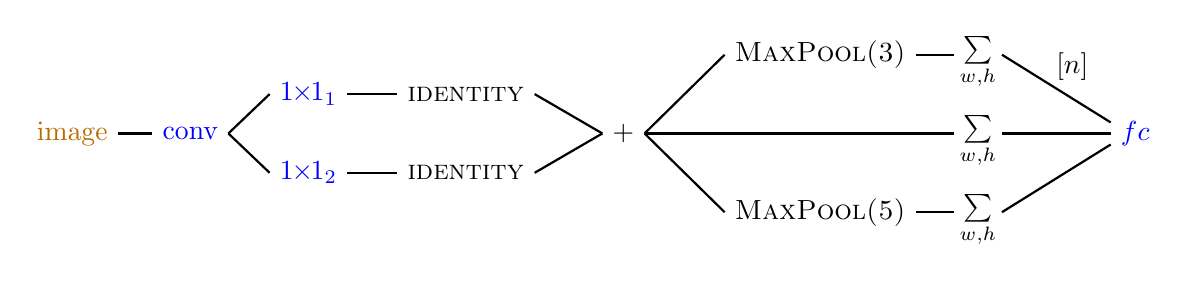
\begin{tikzpicture}
\begin{scope}[
  thick,decoration={
        markings,
        %mark=at position 0.5 with {\arrow{>}}
      }
    ]
\node[text={rgb:red,4;green,2;yellow,1}] (image) at (0,0) {image};
\node[text=blue] (conv) at (1.5, 0) {conv};
\draw[postaction={decorate}] (image.east) -- (conv.west);

\node[text=blue] (a11) at (3, -0.5) {$1\TMS1_2$};
\node[text=blue] (b11) at (3, 0.5) {$1\TMS1_1$};
\draw[postaction={decorate}] (conv.east) -- (a11.west);
\draw[postaction={decorate}] (conv.east) -- (b11.west);

\node (sm_3) at (5.0, -0.5) {\textsc{identity}};
\node (sm_4) at (5.0,  0.5) {\textsc{identity}};
\draw[postaction={decorate}] (a11.east) -- (sm_3.west);
\draw[postaction={decorate}] (b11.east) -- (sm_4.west);


\node (p_2) at (7,  0) {$+$};
\draw[postaction={decorate}] (sm_3.east) -- (p_2.west);
\draw[postaction={decorate}] (sm_4.east) -- (p_2.west);

\node (mp3) at (9.5, 1) {\textsc{MaxPool(3)}};
\node (mp5) at (9.5, -1) {\textsc{MaxPool(5)}};
\draw[postaction={decorate}] (p_2.east) -- (mp3.west);
\draw[postaction={decorate}] (p_2.east) -- (mp5.west);

\node (h_1) at (11.5,  0)  [label={[xshift=0.0cm, yshift=-0.7cm]$\sum\limits_{w,h}$}] {\ \ \ \ };
\node (h_2) at (11.5,  -1)  [label={[xshift=0.0cm, yshift=-0.7cm]$\sum\limits_{w,h}$}] {\ \ \ \ };
\node (h_3) at (11.5,  1)  [label={[xshift=0.0cm, yshift=-0.7cm]$\sum\limits_{w,h}$}] {\ \ \ \ };
%\node (h_1) at (11.5,  0) {$\sum\limits_{w,h}$};
%\node (h_2) at (11.5, -1) {$\sum\limits_{w,h}$};
%\node (h_3) at (11.5,  1) {$\sum\limits_{w,h}$};

\node (num) at (12.7,  0.85) {$[n]$};

\draw[postaction={decorate}] (p_2.east) -- (h_1.west);
\draw[postaction={decorate}] (mp3.east) -- (h_3.west);
\draw[postaction={decorate}] (mp5.east) -- (h_2.west);

\node[text=blue] (fc) at (13.5, 0) {$fc$};
\draw[postaction={decorate}] (h_1.east) -- (fc.west);
\draw[postaction={decorate}]  (h_2.east) -- ([yshift=-4pt] fc.west);
\draw[postaction={decorate}]  (h_3.east) -- ([yshift=4pt] fc.west);

%\path (a11) -- (b11) node [midway, sloped] {$\dots$};
%\path (mp3.south) -- (9.5, 0.10) node [midway, sloped] {$\dots$};

\end{scope}
\end{tikzpicture}
}
\caption{Model data-flow used for All-Pairs.}
\label{typenet_fig_sup}
\end{figure*}

\begin{table}[!htb]
  \centering%
    \begin{tabular}{ l l }
    parameter & value \\
    \hline
    $N_c$ & 4  \\
    $N_f$ & 4  \\
    $N_t$ & 2  \\
    $N_s$ & 3  \\
    $n$ & 64  \\
    \textsc{Ac} & \textsc{Elu}  \\
    \textsc{A} & \textsc{Identity}  \\
    \textsc{Spatial} & \{\textsc{Identity}, \textsc{MaxPool3x3}, \textsc{MaxPool5x5}\}  \\
    \textsc{Afc} & \textsc{Elu}  \\
    \end{tabular}
  \caption{Model level parameters for TypeNet as used to solve All-Pairs.}\label{global_config}
\end{table}

\noindent
For the activation, \textsc{A}$_i$, the most useful activations were found to be \textsc{Identity}, \textsc{Selu}, and
\textsc{SoftMax}.  \textsc{SoftMax} is in the feature, rather than spatial
dimension.  Via architecture search, \textsc{Identity} is the most generally useful activation, though \textsc{SoftMax} tended to reduce training times (probably because it forms a strong approximately-sparse bottleneck).  

The convolution block used \textsc{Elu} activation, no bias, batch norm (post-activation),
and padding to align the convolution filters with the image edges.  It's layer-wise characteristics are detailed below.  For larger images, a stride of 2 was used in \textsc{Conv}$_3$.
\begin{table}[!htb]
  \centering%
    \begin{tabular}{ l l }
    parameter & features, size, stride  \\
    \hline
    \textsc{Conv}$_1$ & 128, 3, 1  \\ 
    \textsc{Conv}$_2$ & 128, 5, 2  \\
    \textsc{Conv}$_3$ & 128, 5, 1  \\
    \textsc{Conv}$_4$ & 128, 3, 1  \\
    \end{tabular}
  \caption{Convolution block parameters for TypeNet as used to solve All-Pairs.}\label{detail_config_1}
\end{table}

\noindent
The fully-connected layers have input of size $m=N_s \TMS n$ and their configuration is detailed below:
\begin{table}[!htb]
  \centering%
    {\renewcommand{\arraystretch}{1.15}
    \begin{tabular}{ l l }
    parameter & value  \\
    \hline
    $fc_1$ & $m$-\textsc{Elu}-bnorm  \\
    $fc_2$ & $\floor*{\frac{m}{2}}$-\textsc{Elu}-bnorm  \\
    $fc_3$ & $\floor*{\frac{m}{4}}$-\textsc{Elu}-bnorm  \\
    $fc_4$ & $2$-\textsc{Identity}  \\
    \end{tabular}
    }
  \caption{Fully-connected parameters for TypeNet as used to solve All-Pairs.}\label{detail_config_2}
\end{table}

\subsection{TypeNet Architecture Search} \label{allpairsresult_sup}

The main hyper-parameters and architecture-variations explored are the
feature activation, number of branches ($k$), and number of features
($n$).  First, we explored the choice of activation with $n=64$ and
$k=2$.  All activation combinations drawn from the following options
were explored and the top results are presented in Figure
\ref{arch_search_fig} : \textsc{Elu} ($\mathsf{E}$), \textsc{Identity} ($\mathsf{I}$), \textsc{Relu} ($\mathsf{R}$), \textsc{Selu} ($\mathsf{Se}$),
\textsc{Sigmoid} ($\mathsf{S}$), \textsc{SoftMax} ($\mathsf{Sm}$), \textsc{SoftPlus} ($\mathsf{Sp}$), and \textsc{Tanh} ($\mathsf{T}$).
In each figure, architectures are labeled with $n$ when $n\neq64$, and the
above abbreviations of the $k$ activations are used.  If a ``$\dashw$'' is appended,
the architecture had a wider convolution receptive field (the stride of the
third \textbf{conv} layer was 2).
%\small
\begin{equation} \label{archnotation_sup:1}
%\mathtt{[n\#-] activation_1 [activation_2 ... activation_k]}.
\mathsf{[\ndash] Activation_1 [... Activation_k]}[\dashw].
\end{equation}
%\normalsize

All of the runs represented in Figure \ref{arch_search_fig} had
higher accuracy than any of the baselines.  The main conclusion from
these trials is that \textsc{SoftMax} and \textsc{Selu} are the most useful
activations.  We most frequently used \textsc{SoftMax} as the activation in
exploring the other hyper-parameters because of its low training
variance.

We studied how the number of branches, $k$, affects training; those
results are shown below with the number of training samples needed to
fully solve the 4-4 All-Pairs problem.  All trials reached 100\% accuracy,
save for one three-branch trial which got stuck at a test accuracy of
99.948\% after 30M training examples.  Based on the number of samples
needed to reach maximum test accuracy, we conclude that $k=2$ is best
for this problem.
\begin{center}
\begin{tabular}{ l l l }
branches ($k$) & accuracy  & training samples \\
\hline
 1 [$\times$9] & $1.0 \pm 0.0$                     & $57.1M \pm 3.8M$ \\
 2 [$\times$10] & $1.0 \pm 0.0$                   & $47.7M \pm 4.7M$    \\
 3 [$\times$20] & $1.0 \pm 10^{-4}$     & $49.4M \pm 8.9M$   \\
%  3 [$\times$20] & $0.99997 \pm 10^{-4}$     & $49.4M \pm 8.9M$   \\
\end{tabular}\label{branches}
\end{center}
The \textsc{SoftMax} activated network with two branches was found to train
faster for more features as summarized in the following table:  \\
\begin{center}
\begin{tabular}{ l l l }
features ($n$) & accuracy  & training samples \\
\hline
 48 [$\times$9] & $1.0 \pm 0.0$       & $57.0M \pm 8.9M$ \\
 64 [$\times$10] & $1.0 \pm 0.0$     & $47.7M \pm 4.7M$    \\
 96 [$\times$20] & $1.0 \pm 0.0$     & $40.5M \pm 7.7M$.   \\
\end{tabular} \\
\end{center}
All options consistently achieved 100\% test accuracy, so this trade-off
for the 4-4 problem can be made to optimize training time or inference
time.

\begin{figure*}[!htb]
\centering
\minipage{0.74\textwidth}
  \includegraphics[width=\linewidth]{images/arch_test_4_4}
\endminipage\hfill
\caption{4-4 All-Pairs for different activation functions, \textsc{A}$_i$.}
\label{arch_search_fig}
\end{figure*}

\subsection{More Details on the Harder All-Pairs Problems}

\begin{figure*}[!htb]
\minipage{0.23\textwidth}
  %\includegraphics[width=\linewidth]{images/missed_examples_77}
  %\includegraphics[width=\linewidth]{images/missed_examples_77_highlight}
  \includegraphics[width=\linewidth]{images/missed_examples_77_highlight_red}
  \endminipage\hfill
\minipage{0.74\textwidth}
  \includegraphics[width=\linewidth]{images/even_harder}
\endminipage\hfill
\caption{\emph{Left}: Examples of incorrect test samples from TypeNet $\mathsf{96{\text -}II{\text -}w}$ trained on 7-7 All-Pairs for 200M samples.  White symbols can be paired, leaving the red symbols unpaired.
  \emph{Right}: Test results of applying TypeNet to more difficult All-Pairs problems.  Wider \textbf{conv} receptive fields are notated with ``-$\mathsf{w}$'', see text for details. }
\label{missed_sup}
\end{figure*}

% ------------------------

The TypeNet approach cannot easily be made to solve every All-Pairs
problem; Figure \ref{missed_sup} shows results for the 5-5, 6-6, and 7-7 All-Pairs problem.
The \textsc{Identity} activation was the only activation to reach 100\% accuracy on the
5-5 and 6-6 problem, in 100\% (Fig\ref{missed_sup}-a) and 20\% (Fig\ref{missed_sup}-d) of trials respectively.  The \textsc{Selu} and \textsc{SoftMax} activation
were not successful on any of these problems in any trail within the 100M
training sample limit.

For these problems, the image size was increased
from $76\TMS76$ to $96\TMS96$ to make room for all the symbols.
This image size increase required decreasing the batch size from 600 to
400; all other training settings remained unchanged.  The large image size led us to expand the receptive field of the \textbf{conv} as notated with ``-$\mathsf{w}$'' and detailed in Section \ref{allpairsresult_sup}.  The most enlightening observations from these experiments are as follows:
\vspace{-4mm}
\begin{tightitemize}
\item The \textsc{Selu} activation (Fig\ref{missed_sup}-c) had lower accuracy
than expected from its effectiveness on the 4-4 problem.
\item On these harder problems, the \textsc{SoftMax} activation continued to
show lower variance across trials in both accuracy and training samples.
\item The $\mathsf{SmSm}$ model (Fig\ref{missed_sup}-b) consistently got stuck
at 94.6\% accuracy on the 5-5 problem, perhaps because the \textsc{SoftMax} activations are prone
to local minima.
\item The number of branches was increased to 3 and number of features to 128,
  independently and together, for the best case activations from smaller models.
  The $\mathsf{128{\text -}III}$ (Fig\ref{missed_sup}-f) model had the best test accuracy, but did worst than the simpler $\mathsf{II}$ model
  (Fig\ref{missed_sup}-e) even when trained to 200M training examples.
\item The 7-7 All-Pairs problem (Fig\ref{missed_sup}-g,h) is clearly
harder. The wider $\mathsf{96{\text -}II{\text -}w}$ (Fig\ref{missed_sup}-g) model was the best.
\item As shown in Figure \ref{missed_sup}-Left, the test samples missed by
one of the $\mathsf{96{\text -}II{\text -}w}$ models on the 7-7 problem are semantically similar: the
model incorrectly labels some samples as $true$ that have either an unpaired
\textbf{cross} and \textbf{3-star}, or an unpaired \textbf{theta} and \textbf{phi}.  For this model and trial, all of its errors fall into these two classes, though it correctly classifies some of those examples (achieving a 95\% accuracy when those two classes account for 9.5\% of the test set).  Different trials show different types of semantic errors.
\item Many variations, including mixtures of activations, more features, more branches, even wider \textbf{conv} receptive fields, and combinations of these choices, were tried to solve the 7-7 problem without success.  In the highest test accuracy observed (98\%), the misclassified images are still easy for a human to classify.
\end{tightitemize}

\subsection{Comparison to a Simple CNN}
\label{comptocnn}
\noindent
Are Lines 5 and 6 of Algorithm 1 generally useful, and do they improve the algorithm?
The table below compares (3 trials for each) the test accuracy and model size of TypeNet with a with a simple convolutional net (ConvNet) created by altering TypeNet as follows:
\begin{itemize}
\item Replace Lines 5 and 6 of Algorithm 1 with \textsc{Flatten} (passing the convolution output directly to the fully-connected layers).
\item As with larger All-Pairs images, use a stride of 2 in \textsc{Conv}$_3$.
\end{itemize}

%\begin{center}
%\begin{tabular}{ r | c c | c c  }
%              & \multicolumn{2}{c|}{ConvNet}                        & \multicolumn{2}{c}{TypeNet}  \\
%dataset  & accuracy & \# parameters & accuracy & \# parameters \\
%\hline
%MNIST               & 0.995167 $\pm$ 0.0004    & 1.39M & \textbf{0.9971 $\pm$ 0.0006} & \textbf{1M}  \\
%Fashion-MNIST & \textbf{0.938133 $\pm$ 0.0008}    & 1.39M & 0.9346 $\pm$ 0.0011 & \textbf{1M} \\
%CIFAR10           & 0.767500 $\pm$ 0.0028     & 1.39M & \textbf{0.8820 $\pm$ 0.0080} & \textbf{1M} \\
%4-4 All-Pairs      & 0.754600 $\pm$ 0.0000     & 3.45M & \textbf{1.0000 $\pm$ 0.0000} & \textbf{1M} \\
%\end{tabular}
%\end{center}

\begin{center}
\begin{tabular}{ r | c c | c c  }
              & \multicolumn{2}{c|}{ConvNet}                        & \multicolumn{2}{c}{TypeNet}  \\
dataset  & accuracy & \# parameters & accuracy & \# parameters \\
\hline
MNIST               & 0.9953 $\pm$ 0.0002    & 2M & \textbf{0.9971 $\pm$ 0.0006} & \textbf{1M}  \\
Fashion-MNIST & \textbf{0.9409 $\pm$ 0.0005}    & 2M & 0.9346 $\pm$ 0.0011 & \textbf{1M} \\
CIFAR10           & 0.7773 $\pm$ 0.0013     & 2.5M & \textbf{0.8820 $\pm$ 0.0080} & \textbf{1M} \\
4-4 All-Pairs      & 0.8080 $\pm$ 0.0925     & 9.9M & \textbf{1.0000 $\pm$ 0.0000} & \textbf{1M} \\
\end{tabular}
\end{center}

\noindent
From this comparison, TypeNet is seen to have fewer parameters and shows significant improvements in accuracy for the hardest two datasets (CIFAR10 and 4-4 All-Pairs).  The number of parameters in TypeNet is not dependent on the input size because of the spatial summation in Line 6 of the algorithm.  We anticipate the spatial, learned histogram of TypeNet to be a useful tool in the construction of other DNN architectures.

%\raggedbottom
%\vfill



\end{document}
